%%%%%%%%%%%%%%%%%%%%%%%%%%%%%%%%%%%%%%%%
% datoteka diploma-FRI-vzorec.tex
%
% vzorčna datoteka za pisanje diplomskega dela v formatu LaTeX
% na UL Fakulteti za računalništvo in informatiko
%
% na osnovi starejših verzij vkup spravil Franc Solina, maj 2021
% prvo verzijo je leta 2010 pripravil Gašper Fijavž
%
% za upravljanje z literaturo ta vezija uporablja BibLaTeX
%
% svetujemo uporabo Overleaf.com - na tej spletni implementaciji LaTeXa ta vzorec zagotovo pravilno deluje
%

\documentclass[a4paper,12pt,openright]{book}
%\documentclass[a4paper, 12pt, openright, draft]{book}  Nalogo preverite tudi z opcijo draft, ki pokaže, katere vrstice so predolge! Pozor, v draft opciji, se slike ne pokažejo!
 
\usepackage[utf8]{inputenc}   % omogoča uporabo slovenskih črk kodiranih v formatu UTF-8
\usepackage[slovene,english]{babel}    % naloži, med drugim, slovenske delilne vzorce
\usepackage[pdftex]{graphicx}  % omogoča vlaganje slik različnih formatov
\usepackage{fancyhdr}          % poskrbi, na primer, za glave strani
\usepackage{amssymb}           % dodatni matematični simboli
\usepackage{amsmath}           % eqref, npr.
\usepackage[hyphens]{url}
\usepackage{csquotes}
\usepackage[pdftex, colorlinks=true,
						citecolor=black, filecolor=black, 
						linkcolor=black, urlcolor=black,
						pdfproducer={LaTeX}, pdfcreator={LaTeX}]{hyperref}
\usepackage{hyperxmp}
\usepackage{color}
\usepackage{soul}

\usepackage{caption}
\usepackage{subcaption}

\usepackage[table,dvipsnames]{xcolor}
\usepackage{tabularx}
\usepackage{listings}
\renewcommand{\lstlistingname}{Izvorna koda}
%\lstset{
%  basicstyle=\fontsize{11}{13}\selectfont\ttfamily
%}
\lstdefinestyle{mystyle}{
  %commentstyle=\color{codegreen},
  keywordstyle=\color{magenta},
  %numberstyle=\tiny\color{codegray},
  stringstyle=\color{codepurple},
  basicstyle=\ttfamily\footnotesize,
  breakatwhitespace=false,         
  breaklines=true,                 
  captionpos=b,                    
  keepspaces=true,                 
  numbers=left,                    
  numbersep=5pt,                  
  showspaces=false,                
  showstringspaces=false,
  showtabs=false,                  
  tabsize=2
}
\lstset{style=mystyle}

\usepackage[
backend=bibtex,
style=numeric,
sorting=nty,
]{biblatex}


\addbibresource{literatura.bib} %Imports bibliography file


%%%%%%%%%%%%%%%%%%%%%%%%%%%%%%%%%%%%%%%%
%	DIPLOMA INFO
%%%%%%%%%%%%%%%%%%%%%%%%%%%%%%%%%%%%%%%%
\newcommand{\ttitle}{Inženiring vzporednih algoritmov}
\newcommand{\ttitleEn}{Parallel Algorithm Engineering}
\newcommand{\tsubject}{\ttitle}
\newcommand{\tsubjectEn}{\ttitleEn}
\newcommand{\tauthor}{Luka Bajić}
\newcommand{\tkeywords}{vzporedni algoritmi, večnitnost, Levenshteinova razdalja, LCS}
\newcommand{\tkeywordsEn}{computer, computer, computer}

%%%%%%%%%%%%%%%%%%%%%%%%%%%%%%%%%%%%%%%%
%	HYPERREF SETUP
%%%%%%%%%%%%%%%%%%%%%%%%%%%%%%%%%%%%%%%%
\hypersetup{pdftitle={\ttitle}}
\hypersetup{pdfsubject=\ttitleEn}
\hypersetup{pdfauthor={\tauthor}}
\hypersetup{pdfkeywords=\tkeywordsEn}

%%%%%%%%%%%%%%%%%%%%%%%%%%%%%%%%%%%%%%%%
% postavitev strani
%%%%%%%%%%%%%%%%%%%%%%%%%%%%%%%%%%%%%%%%  

\addtolength{\marginparwidth}{-20pt} % robovi za tisk
\addtolength{\oddsidemargin}{40pt}
\addtolength{\evensidemargin}{-40pt}

\renewcommand{\baselinestretch}{1.3} % ustrezen razmik med vrsticami
\setlength{\headheight}{15pt}        % potreben prostor na vrhu
\renewcommand{\chaptermark}[1]%
{\markboth{\MakeUppercase{\thechapter.\ #1}}{}} \renewcommand{\sectionmark}[1]%
{\markright{\MakeUppercase{\thesection.\ #1}}} \renewcommand{\headrulewidth}{0.5pt} \renewcommand{\footrulewidth}{0pt}
\fancyhf{}
\fancyhead[LE,RO]{\sl \thepage} 
%\fancyhead[LO]{\sl \rightmark} \fancyhead[RE]{\sl \leftmark}
\fancyhead[RE]{\sc \tauthor}              % dodal Solina
\fancyhead[LO]{\sc Diplomska naloga}     % dodal Solina


\newcommand{\BibLaTeX}{{\sc Bib}\LaTeX}
\newcommand{\BibTeX}{{\sc Bib}\TeX}

%%%%%%%%%%%%%%%%%%%%%%%%%%%%%%%%%%%%%%%%
% naslovi
%%%%%%%%%%%%%%%%%%%%%%%%%%%%%%%%%%%%%%%%  

\newcommand{\autfont}{\Large}
\newcommand{\titfont}{\LARGE\bf}
\newcommand{\clearemptydoublepage}{\newpage{\pagestyle{empty}\cleardoublepage}}
\setcounter{tocdepth}{1}	      % globina kazala

%%%%%%%%%%%%%%%%%%%%%%%%%%%%%%%%%%%%%%%%
% konstrukti
%%%%%%%%%%%%%%%%%%%%%%%%%%%%%%%%%%%%%%%%  
\newtheorem{izrek}{Izrek}[chapter]
\newtheorem{trditev}{Trditev}[izrek]
\newenvironment{dokaz}{\emph{Dokaz.}\ }{\hspace{\fill}{$\Box$}}


%%%%%%%%%%%%%%%%%%%%%%%%%%%%%%%%%%%%%%%%%%%%%%%%%%%%%%%%%%%%%%%%%%%%%%%%%%%%%%%
%% PDF-A
%%%%%%%%%%%%%%%%%%%%%%%%%%%%%%%%%%%%%%%%%%%%%%%%%%%%%%%%%%%%%%%%%%%%%%%%%%%%%%%

%%%%%%%%%%%%%%%%%%%%%%%%%%%%%%%%%%%%%%%% 
% define medatata
%%%%%%%%%%%%%%%%%%%%%%%%%%%%%%%%%%%%%%%% 
\def\Title{\ttitle}
\def\Author{\tauthor, lb4129@student.uni-lj.si}
\def\Subject{\ttitleEn}
\def\Keywords{\tkeywordsEn}

%%%%%%%%%%%%%%%%%%%%%%%%%%%%%%%%%%%%%%%% 
% \convertDate converts D:20080419103507+02'00' to 2008-04-19T10:35:07+02:00
%%%%%%%%%%%%%%%%%%%%%%%%%%%%%%%%%%%%%%%% 
\def\convertDate{%
    \getYear
}

{\catcode`\D=12
 \gdef\getYear D:#1#2#3#4{\edef\xYear{#1#2#3#4}\getMonth}
}
\def\getMonth#1#2{\edef\xMonth{#1#2}\getDay}
\def\getDay#1#2{\edef\xDay{#1#2}\getHour}
\def\getHour#1#2{\edef\xHour{#1#2}\getMin}
\def\getMin#1#2{\edef\xMin{#1#2}\getSec}
\def\getSec#1#2{\edef\xSec{#1#2}\getTZh}
\def\getTZh +#1#2{\edef\xTZh{#1#2}\getTZm}
\def\getTZm '#1#2'{%
    \edef\xTZm{#1#2}%
    \edef\convDate{\xYear-\xMonth-\xDay T\xHour:\xMin:\xSec+\xTZh:\xTZm}%
}

%\expandafter\convertDate\pdfcreationdate 

%%%%%%%%%%%%%%%%%%%%%%%%%%%%%%%%%%%%%%%%
% get pdftex version string
%%%%%%%%%%%%%%%%%%%%%%%%%%%%%%%%%%%%%%%% 
\newcount\countA
\countA=\pdftexversion
\advance \countA by -100
\def\pdftexVersionStr{pdfTeX-1.\the\countA.\pdftexrevision}


%%%%%%%%%%%%%%%%%%%%%%%%%%%%%%%%%%%%%%%%
% XMP data
%%%%%%%%%%%%%%%%%%%%%%%%%%%%%%%%%%%%%%%%  
\usepackage{xmpincl}
%\includexmp{pdfa-1b}

%%%%%%%%%%%%%%%%%%%%%%%%%%%%%%%%%%%%%%%%
% pdfInfo
%%%%%%%%%%%%%%%%%%%%%%%%%%%%%%%%%%%%%%%%  
\pdfinfo{%
    /Title    (\ttitle)
    /Author   (\tauthor, lb4129@student.uni-lj.si)
    /Subject  (\ttitleEn)
    /Keywords (\tkeywordsEn)
    /ModDate  (\pdfcreationdate)
    /Trapped  /False
}

%%%%%%%%%%%%%%%%%%%%%%%%%%%%%%%%%%%%%%%%
% znaki za copyright stran
%%%%%%%%%%%%%%%%%%%%%%%%%%%%%%%%%%%%%%%%  

\newcommand{\CcImageCc}[1]{%
	
\includegraphics[scale=#1]{cc_cc_30.pdf}%
}
\newcommand{\CcImageBy}[1]{%
	
\includegraphics[scale=#1]{cc_by_30.pdf}%
}
\newcommand{\CcImageSa}[1]{%
	
\includegraphics[scale=#1]{cc_sa_30.pdf}%
}

%%%%%%%%%%%%%%%%%%%%%%%%%%%%%%%%%%%%%%%%%%%%%%%%%%%%%%%%%%%%%%%%%%%%%%%%%%%%%%%
%%%%%%%%%%%%%%%%%%%%%%%%%%%%%%%%%%%%%%%%%%%%%%%%%%%%%%%%%%%%%%%%%%%%%%%%%%%%%%%

\begin{document}
\selectlanguage{slovene}
\frontmatter
\setcounter{page}{1} %
\renewcommand{\thepage}{}       % preprečimo težave s številkami strani v kazalu

%%%%%%%%%%%%%%%%%%%%%%%%%%%%%%%%%%%%%%%%
%naslovnica
 \thispagestyle{empty}%
   \begin{center}
    {\large\sc Univerza v Ljubljani\\%
%      Fakulteta za elektrotehniko\\% za študijski program Multimedija
%      Fakulteta za upravo\\% za študijski program Upravna informatika
      Fakulteta za računalništvo in informatiko\\%
%      Fakulteta za matematiko in fiziko\\% za študijski program Računalništvo in matematika
     }
    \vskip 10em%
    {\autfont \tauthor\par}%
    {\titfont \ttitle \par}%
    {\vskip 3em \textsc{DIPLOMSKO DELO\\[5mm]         % dodal Solina za ostale študijske programe
%    VISOKOŠOLSKI STROKOVNI ŠTUDIJSKI PROGRAM\\ PRVE STOPNJE\\ RAČUNALNIŠTVO IN INFORMATIKA}\par}%
     VISOKOŠOLSKI  ŠTUDIJSKI PROGRAM\\ PRVE STOPNJE\\ RAČUNALNIŠTVO IN INFORMATIKA}\par}%
%    INTERDISCIPLINARNI UNIVERZITETNI\\ ŠTUDIJSKI PROGRAM PRVE STOPNJE\\ MULTIMEDIJA}\par}%
%    INTERDISCIPLINARNI UNIVERZITETNI\\ ŠTUDIJSKI PROGRAM PRVE STOPNJE\\ UPRAVNA INFORMATIKA}\par}%
%    INTERDISCIPLINARNI UNIVERZITETNI\\ ŠTUDIJSKI PROGRAM PRVE STOPNJE\\ RAČUNALNIŠTVO IN MATEMATIKA}\par}%
    \vfill\null%
% izberite pravi habilitacijski naziv mentorja!
    {\large \textsc{Mentor}: doc. dr. Jurij Mihelič\par}%
   %{\large \textsc{Somentor}:  viš. pred./doc./izr. prof./prof. dr.  Martin Krpan \par}%
    {\vskip 2em \large Ljubljana, \the\year \par}%
\end{center}
% prazna stran
%\clearemptydoublepage      
% izjava o licencah itd. se izpiše na hrbtni strani naslovnice

%%%%%%%%%%%%%%%%%%%%%%%%%%%%%%%%%%%%%%%%
%copyright stran
%%%%%%%%%%%%%%%%%%%%%%%%%%%%%%%%%%%%%%%%
\newpage
\thispagestyle{empty}

\vspace*{5cm}
{\small \noindent
To delo je ponujeno pod licenco \textit{Creative Commons Priznanje avtorstva-Deljenje pod enakimi pogoji 2.5 Slovenija} (ali novej\v so razli\v cico).
To pomeni, da se tako besedilo, slike, grafi in druge sestavine dela kot tudi rezultati diplomskega dela lahko prosto distribuirajo,
reproducirajo, uporabljajo, priobčujejo javnosti in predelujejo, pod pogojem, da se jasno in vidno navede avtorja in naslov tega
dela in da se v primeru spremembe, preoblikovanja ali uporabe tega dela v svojem delu, lahko distribuira predelava le pod
licenco, ki je enaka tej.
Podrobnosti licence so dostopne na spletni strani \href{http://creativecommons.si}{creativecommons.si} ali na Inštitutu za
intelektualno lastnino, Streliška 1, 1000 Ljubljana.

\vspace*{1cm}
\begin{center}% 0.66 / 0.89 = 0.741573033707865
\CcImageCc{0.741573033707865}\hspace*{1ex}\CcImageBy{1}\hspace*{1ex}\CcImageSa{1}%
\end{center}
}

\vspace*{1cm}
{\small \noindent
Izvorna koda diplomskega dela, njeni rezultati in v ta namen razvita programska oprema je ponujena pod licenco GNU General Public License,
različica 3 (ali novejša). To pomeni, da se lahko prosto distribuira in/ali predeluje pod njenimi pogoji.
Podrobnosti licence so dostopne na spletni strani \url{http://www.gnu.org/licenses/}.
}

\vfill
\begin{center} 
\ \\ \vfill
{\em
Besedilo je oblikovano z urejevalnikom besedil \LaTeX.}
\end{center}

% prazna stran
\clearemptydoublepage

%%%%%%%%%%%%%%%%%%%%%%%%%%%%%%%%%%%%%%%%
% stran 3 med uvodnimi listi
\thispagestyle{empty}
\
\vfill

\bigskip
\noindent\textbf{Kandidat:} Luka Bajić\\
\noindent\textbf{Naslov:} Inženiring vzporednih algoritmov\\
% vstavite ustrezen naziv študijskega programa!
\noindent\textbf{Vrsta naloge:} Diplomska naloga na visokošolskem programu prve stopnje Računalništvo in informatika \\
% izberite pravi habilitacijski naziv mentorja!
\noindent\textbf{Mentor:} doc. dr. Jurij Mihelič\\
%\noindent\textbf{Somentor:} isto kot za mentorja

\bigskip
\noindent\textbf{Opis:}\\
V diplomski nalogi \cite{diplomaPremk} je študent preizkusil različne tehnike za povzporejanje algoritma za izračun DTW (dynamic time warping) razdalje, ki sem jih nato še dopolnil. Predvidevam, da bi enake tehnike bile uporabne tudi za nekatere druge probleme, kot je razdalja LCS (longest common subsequence) ali Levenshteinova razdalja. V nalogi je torej treba te tehnike sprogramirati za omenjena problema (lahko le en problem, če bo veliko dela), nato pa jih smiselno eksperimentalno ovrednotiti.

%\bigskip
%\noindent\textbf{Title:} Parallel algorithm engineering
%\bigskip
%\noindent\textbf{Description:}\\
%opis diplome v angleščini

\vfill

\vspace{2cm}

% prazna stran
\clearemptydoublepage

% zahvala
\thispagestyle{empty}\mbox{}\vfill\null\it%
\noindent
Zahvaljujem se mentorju doc. dr. Juriju Miheliču za pomoč pri izdelavi diplomske naloge in Urošu Koritniku za moralno podporo in koristne nasvete tekom študija. 
\rm\normalfont

% prazna stran
\clearemptydoublepage

%%%%%%%%%%%%%%%%%%%%%%%%%%%%%%%%%%%%%%%%
% posvetilo, če sama zahvala ne zadošča :-)
\thispagestyle{empty}\mbox{}{\vskip0.20\textheight}\mbox{}\hfill\begin{minipage}{0.55\textwidth}%
%Svoji dragi Alenčici.
\normalfont\end{minipage}

% prazna stran
\clearemptydoublepage

%%%%%%%%%%%%%%%%%%%%%%%%%%%%%%%%%%%%%%%%
% kazalo
\pagestyle{empty}
\def\thepage{}% preprečimo težave s številkami strani v kazalu
\tableofcontents{}

% prazna stran
\clearemptydoublepage

%%%%%%%%%%%%%%%%%%%%%%%%%%%%%%%%%%%%%%%%
% seznam kratic

\chapter*{Seznam uporabljenih kratic}

\noindent\begin{tabular}{p{0.11\textwidth}|p{.39\textwidth}|p{.39\textwidth}}    % po potrebi razširi prvo kolono tabele na račun drugih dveh!
  {\bf kratica} & {\bf angleško}                              & {\bf slovensko} \\ \hline
  {\bf LCS}      & longest common subsequence               & najdaljše skupno podzaporedje \\
  {\bf JSON} & JavaScript Object Notation & JavaScript objektna notacija \\
%  \dots & \dots & \dots \\
\end{tabular}

% prazna stran
\clearemptydoublepage

%%%%%%%%%%%%%%%%%%%%%%%%%%%%%%%%%%%%%%%%
% povzetek
\phantomsection
\addcontentsline{toc}{chapter}{Povzetek}
\chapter*{Povzetek}

\noindent\textbf{Naslov:} \ttitle
\bigskip

\noindent\textbf{Avtor:} \tauthor
\bigskip

%\noindent\textbf{Povzetek:} 
\noindent Algoritmi za iskanje podobnosti med nizi so pomemben gradnik raznovrstnih aplikacij, ki so dandanes v vsakodnevni uporabi, od črkovalnikov do orodij za kontrolo različic (npr. Git). Diplomsko delo opiše različne pristope optimizacije dveh tovrstnih algoritmov: Levenshteinove razdalje in najdaljšega skupnega podzaporedja, z uporabo koncepta večnitnosti in dveh temeljnjih pristopov paralelizacije - diagonalni in naprej-nazaj. Glavni cilj je časovna pohitritev algoritmov, ki jo ustrezno izmerimo in primerjamo nove implementacije z obstoječimi. Za pristop naprej-nazaj razvijemo tudi prostorsko optimizirano metodo, ki je smiselna za uporabo pri ogromnih količinah vhodnih podatkov. 

\bigskip

\noindent\textbf{Ključne besede:} \tkeywords.
% prazna stran
\clearemptydoublepage

%%%%%%%%%%%%%%%%%%%%%%%%%%%%%%%%%%%%%%%%
% abstract
\phantomsection
\selectlanguage{english}
\addcontentsline{toc}{chapter}{Abstract}
\chapter*{Abstract}

\noindent\textbf{Title:} \ttitleEn
\bigskip

\noindent\textbf{Author:} \tauthor
\bigskip

%\noindent\textbf{Abstract:} 
\noindent Algorithms for finding similarity between strings are a building block of a large variety of modern applications, from spell checkers to version control tools (e.g. Git). This BSc thesis describes various approaches for optimizing two such algorithms: Levenshtein distance and Longest Common Subsequence, utilizing the concept of multithreading and two fundamental parallelization approaches - diagonal and forward-backward. Main objective is improved execution time of said algorithms, which we measure and compare our results with existing implementations. For forward-backward apporach we develop an additional space optimization, which is useful for extremely large amounts of input data.

\bigskip

\noindent\textbf{Keywords:} \tkeywordsEn.
\selectlanguage{slovene}
% prazna stran
\clearemptydoublepage

%%%%%%%%%%%%%%%%%%%%%%%%%%%%%%%%%%%%%%%%
\mainmatter
\setcounter{page}{1}
\pagestyle{fancy}

\chapter{Uvod}

V diplomskem delu so opisani različni pristopi za optimizacijo algoritmov za računanje Levenshteinove razdalje in najdaljšega skupnega podzaporedja (angl. Longest Common Subsequence - LCS) z uporabo vzporednega procesiranja. Gre za dva zelo pogosto uporabljena algoritma za potrebe primerjave nizov oziroma iskanje razdalje med nizi, ki ju običajno rešujemo z dinamičnim programiranjem (za potrebe tega diplomskega dela smo se omejili na razdalje med točno dvema nizoma, ki je tudi najpogosteje uporabljena v praktičnih aplikacijah). S pomočjo koncepta večnitnosti smo razvili več različic algoritmov, ki dosežejo časovno pohitritev v primerjavi z osnovno implementacijo. Pri tem smo uporabili dva različna načina povzporejanja: diagonalni in naprej-nazaj. Meritve smo izvajali na naključno generiranih nizih, velikosti med 10000 in 400000 znakov. Poleg časovne pohitritve, smo iskali tudi možnosti za prostorske optimizacije, torej algoritme, ki zasedejo čimmanjšo količino delovnega pomnilnika, kar je uporabno predvsem za vhodne podatke ogromne velikosti, ki jih ni smiselno, oziroma pogosto celo nemogoče v celoti hraniti v delovnem pomnilniku. 

\section{Motivacija}

Iskanje podobnosti med nizi se na prvi pogled zdi dokaj enostaven problem, vendar gre v resnici za obsežno in raznoliko skupino algoritmov, ki služijo kot gradniki aplikacij na številnih področjih in v različnih domenah, v katerih se običajno srečujemo z zelo specifičnimi potrebami oz. zahtevami. Tipičen primer je bioinformatika ali genetika \cite{LCSpracticalUse}, kjer pogosto naletimo na probleme z ozkim naborom znakov in lahko algoritme temu primerno tudi prilagodimo. Kot drugi primer vzamemo orodja za kontrolo različic \cite{levenshteinMotivation}. Tukaj lahko pričakujemo, da bosta dve datoteki, ki ju primerjamo, večinoma zelo podobni, morda samo z nekaj spremenjenimi vrsticami, posledično lahko razvijemo algoritem, ki bo tovrstna pričakovanja upošteval in se morda na nek način obnašal bolj uporabniku prijazno (npr. z nekimi hitrimi, vmesnimi aproksimacijami, če je celotno izvajanje preveč dolgotrajno). 

Iz tovrstnih praktičnih uporab vidimo, da je vsaka optimizacija algoritmov za iskanje razdalje med nizi zelo koristna, zato smo v tem diplomskem delu preučili nekaj tovrstnih pristopov za algoritma za računanje LCS in Levenshteinove razdalje. Omenjeni primeri so sicer zelo odvisni od specifične domene, v našem delu pa smo se osredotočili na iskanje splošnih rešitev, ki pridejo v poštev ne glede na tip vhodnih podatkov, predpostavljamo samo, da naprava na kateri algoritme izvajamo, omogoča večnitnost. 

\section{Struktura}

Diplomsko delo je razdeljeno na pet poglavij. Po uvodnem delu sledi opis obeh temeljnjih algoritmov, njune praktične uporabnosti in njunih implementacij z uporabo dinamičnega programiranja. Tretje poglavje predstavi dva glavna pristopa povzporejanja - diagonalni in naprej-nazaj. Pri diagonalnem je predstavljen tudi način optimizacije prenosov iz glavnega pomnilnika v predpomnilnik, ki je dejansko ključen za hitro delovanje algoritma. Poleg tega za vsako implementacijo opišemo še primer prostorske optimizacije. V četrtem poglavju so predstavljeni rezultati meritev na različnih velikostih vhodnih podatkov in primerjave časov izvajanja posameznih različic algoritmov. V petem poglavju sledijo še sklepne ugotovitve in morebitne ideje za nadaljnji razvoj. 

\chapter{Metode in paradigme}

V tem poglavju je predstavljena algoritmična paradigma dinamičnega programiranja, ki služi kot temelj za vse algoritme, ki so predstavljeni v nadaljevanju. Nato sta podrobneje opisana še osnovna algoritma za računanje LCS in Levenshteinove razdalje. 

\section{Dinamično programiranje}

Dinamično programiranje je algoritmična paradigma, s katero skušamo optimizirati izvajanje problemov, ki imajo takoimenovano optimalno podstrukturo, kar pomeni, da je do rešitve problema možno priti preko optimalne rešitve njihovih podproblemov. Za to obstajata dva glavna načina: rekurzivni (z uporabo memoizacije) in iterativni (z uporabo tabeliranja). Za našo implementacijo smo uporabili iterativni pristop, kar pomeni, da hranimo vmesne rezultate v tabeli velikosti $n \times m$. Problem primerjanja dveh nizov smo tako razbili na enostavnejše podprobleme primerjanja dveh znakov. Končni rezultat se nahaja v celici $(n,m)$, vendar lahko iz preostanka tabele tudi rekonstruiramo pot, po kateri smo prišli do rezultata. 

\section{Levenshteinova razdalja}

Predpostavimo, da lahko nad vsakim znakom v nizu izvedemo tri osnovne operacije: brisanje, vstavljanje in spreminjanje. Hipotetično lahko posameznim operacijam dodelimo tudi uteži \cite{weightedLevenshtein}, vendar ker to nima občutnega vpliva na časovno zahtevnost algoritma, v nadaljevanju sklepamo, da imajo vse tri enako utež. S tem naborom operacij obstaja teoretično neskončno možnih načinov za transformacijo nekega niza v poljuben drugi niz, Levenshteinova razdalja pa predstavlja dolžino najkrajše tovrstne transformacije. 

Izračunamo jo tako, da najprej inicializiramo prvo vrstico in stolpec matrike. Ker gre tukaj dejansko za primerjavo niza s praznim nizom, je ta korak trivialen in vedno enak: v prvo vrstico vnesemo vrednosti spremenljivke $j$, v prvi stolpec pa vrednosti spremenljivke $i$, kot je prikazano na sliki (\ref{levenshteinExample}) v rdečem fontu.

\begin{figure}[htb]
\begin{center}
\begin{tabular}{|l|l|l|l|l|l|}
\cline{3-6}
  \multicolumn{2}{c|}{}  & a & b & c & d\\ \cline{2-6}
 \multicolumn{1}{c|}{} & \textcolor{red}{0} & \textcolor{red}{1} & \textcolor{red}{2} & \textcolor{red}{3} & \textcolor{red}{4}\\ \hline
x  & \textcolor{red}{1}  & \cellcolor{blue!15}1 &  2 & 3 & 4\\ \hline
y  & \textcolor{red}{2} & 2 & \cellcolor{blue!15}2 & 3 & 4\\ \hline
z  & \textcolor{red}{3} & 3 & 3 & \cellcolor{blue!15}3 & \cellcolor{blue!25}4 \\ \hline
\end{tabular}

\end{center}
\caption{Primer izračunane matrike za iskanje Levenshteinove razdalje za dva naključna niza}
\label{levenshteinExample}
\end{figure}

Nato vrednosti za preostale celice v matriki izračunamo po formuli (\ref{LevenshteinEquation}), za $i=1,...,n$ in $j=1,...,m$, kjer $s1$ in $s2$ predstavljata vhodna niza dolžin $n$ in $m$. Končni rezultat dobimo v celici na poziciji $(n, m)$. 

\bigskip \bigskip

\begin{equation}
\label{LevenshteinEquation}
\begin{aligned}
M(i, j) =
\begin{cases}
     M(i-1, j-1) ,     \\ \quad \quad \quad \text{če } s1[i-1]=s2[j-1]\\
     1 + min(M(i, j-1), min(M(i-1, j), M(i-1, j-1))) , \\ \quad \quad \quad \text{če } s1[i-1] \neq s2[j-1]
  \end{cases}
\end{aligned}
\end{equation}

\bigskip \bigskip

Sama implementacija je precej intuitivna - z dvojno zanko iteriramo po globalni tabeli in računamo vrednosti po formuli glede na enakost trenutnih dveh znakov v vhodnih nizih $str1$ in $str2$, pri čemer moramo biti pozorni, da pri indeksiranju upoštevamo dodatno vrstico in stolpec, ki smo ju vstavili za inicializacijo začetnih vrednosti (vrstica 8 v kodi \ref{LevenshteinNaprej}). \bigskip \bigskip

\begin{lstlisting}[language=C++, caption={Algoritem za izračun Levenshteinove razdalje}, captionpos=b, label=LevenshteinNaprej]
int forward_levenshtein (string str1, string str2, int row, int column) {
    for(int i = 0; i < row; i++) {
        for (int j = 0; j < column; j++) {    
            if (i == 0)
                arr[i][j] = j;
            else if (j == 0)
                arr[i][j] = i;
            else if (str1[i-1] == str2[j-1])
                arr[i][j] = arr[i-1][j-1];
            else 
                arr[i][j] = 1 + min(arr[i][j-1], min(arr[i-1][j], arr[i-1][j-1]));
        }
    }

    return arr[row][column];
}
\end{lstlisting}

\subsection{Primer uporabe}

Avtorja članka \cite{documentsimilarity} sta razvila svojo zgoščevalno funkcijo za potrebe primerjanja podobnosti med dvema datotekama. Ideja je, da algoritem datoteki, ki sta potencialno dolžine več megabajtov, skrči na neko manjšo velikost (npr. nekaj kilobajtov) in na koncu nad tema krajšima reprezentacijama požene iskanje Levenshteinove razdalje. Dejansko gre torej za aproksimacijo razlike oz. podobnosti med datotekama, vendar se izkaže, da je ta zadnji korak (torej dejansko iskanje podobnosti) kljub vsemu ozko grlo celotnega procesa, tako da je čimbolj optimalna implementacija algoritma za iskanje Levenshteinove razdalje ključnega pomena. 

\section{LCS}

Podsekvenco definiramo kot zaporedje znakov, ki se nahajajo v nizu, v istem vrstnem redu, vendar ne nujno zaporedno. Torej, niz $"ABCD"$ vsebuje podsekvenco $"ACD"$, ne vsebuje pa podsekvence $"DCB"$. Najdaljša skupna podsekvenca, oziroma LCS, predstavlja najdaljšo možno podsekvenco, ki se nahaja v dveh (ali več \cite{LCSmultipleSequences}) vhodnih nizih, v naših algoritmih pa iščemo dolžino te podsekvence. 

Pristop reševanja tega problema je podoben kot za Levenshteinovo razdaljo v prejšnjem poglavju: začetne vrednosti za prvo vrstico in prvi stolpec so v tem primeru kar ničle, saj je pri praznem nizu dolžina podsekvence vedno 0. Preostanek tabele pa izračunamo po formuli (\ref{LCSequation}), za $i=1,...,n$ in $j=1,...,m$, kjer $s1$ in $s2$ predstavljata vhodna niza dolžin $n$ in $m$. Končni rezultat ponovno dobimo v celici $(n, m)$, kot je prikazano na sliki \ref{LCSexample}. 

\begin{equation}
\label{LCSequation}
\begin{aligned}
M(i, j) = 
\begin{cases}
     1 + M(i-1, j-1) ,      \\ \quad \quad \quad\text{če } s1[i-1]=s2[j-1]\\
     max(M(i-1, j), M(i, j-1)) , \\ \quad \quad \quad \text{če } s1[i-1] \neq s2[j-1]
  \end{cases}
\end{aligned}
\end{equation}

\bigskip \bigskip

\begin{figure}[htb]
\begin{center}
\begin{tabular}{|l|l|l|l|l|l|}
\cline{3-6}
  \multicolumn{2}{c|}{}  & a & b & c & d\\ \cline{2-6}
 \multicolumn{1}{c|}{} & \textcolor{red}{0} & \textcolor{red}{0} & \textcolor{red}{0} & \textcolor{red}{0} & \textcolor{red}{0}\\ \hline
b  & \textcolor{red}{0} & 0 & \cellcolor{blue!15}1 & 1 & 1\\ \hline
c  & \textcolor{red}{0} & 0 & 1 & \cellcolor{blue!15}2 & \cellcolor{blue!15}2\\ \hline
a  & \textcolor{red}{0} & 1 & 1 & 2 & \cellcolor{blue!25}2 \\ \hline
\end{tabular}
\end{center}
\caption{Primer izračunane matrike za iskanje LCS za dva naključna niza}
\label{LCSexample}
\end{figure}

Implementacija algoritma je prav tako podobna Levenshteinovi (\ref{LevenshteinNaprej}), razlika je le v formuli za izračun vrednosti v posameznih celicah. V tem primeru bi lahko celo izpustili inicializacijo začetnih vrednosti (vrstici 4 in 5 v kodi \ref{LCSnaprej}), če bi bili prepričani, da je prazna tabela že predhodno napolnjena z ničlami. 

\bigskip \bigskip

\begin{lstlisting}[language=C++, caption={Algoritem za izračun LCS}, captionpos=b, label=LCSnaprej]
int forward_LCS (string str1, string str2, int row, int column) {
    for(int i = 0; i < row; i++) 
        for (int j = 0; j < column; j++) 
            if (i == 0 || j == 0)
                arr[i][j] = 0;
            else if (str1[i-1] == str2 [j-1])
                arr[i][j] = 1 + arr[i-1][j-1];
            else
                arr[i][j] = max(arr[i-1][j], arr[i][j-1]);

    return arr[row][column];
}
\end{lstlisting}

\chapter{Vzporedni algoritmi}

Osnovna struktura vzporednega algoritma za oba problema je enaka kot njuna rešitev iz prejšnjega poglavja - še vedno uporabljamo dvodimenzionalno tabelo za hranjenje vmesnih vrednosti, torej je prostorska zahtevnost enaka - $O(n \times m)$. Razlika je samo v tem, da vrednosti, ki niso medsebojno odvisne, lahko računamo vzporedno z uporabo koncepta večnitnosti (angl. multithreading). Za to obstajata dva glavna pristopa - diagonalni in naprej-nazaj. Poleg tega smo razvili tudi prostorsko optimizirane algoritme, ki ne hranijo celotne tabele v pomnilniku, temveč samo trenutno in prejšnjo vrstico. 

Vsega skupaj smo implementirali 20 različic algoritmov:
\begin{itemize}
  \item LCS naprej 
  \item LCS naprej s prostorsko optimizacijo
  \item LCS nazaj 
  \item LCS nazaj s prostorsko optimizacijo
  \item LCS naprej-nazaj (2 niti)
  \item LCS naprej-nazaj s prostorsko optimizacijo (2 niti)
  \item LCS diagonalno
  \item LCS diagonalno s prostorsko optimizacijo
  \item LCS diagonalno vzporedno (poljubno število niti)
  \item LCS diagonalno vzporedno s prostorsko optimizacijo (poljubno število niti)
  \item Levenshteinova razdalja naprej 
  \item Levenshteinova razdalja naprej s prostorsko optimizacijo
  \item Levenshteinova razdalja nazaj 
  \item Levenshteinova razdalja nazaj s prostorsko optimizacijo
  \item Levenshteinova razdalja naprej-nazaj (2 niti)
  \item Levenshteinova razdalja naprej-nazaj s prostorsko optimizacijo (2 niti)
  \item Levenshteinova razdalja diagonalno
  \item Levenshteinova razdalja diagonalno s prostorsko optimizacijo
  \item Levenshteinova razdalja diagonalno vzporedno (poljubno število niti)
  \item Levenshteinova razdalja diagonalno vzporedno s prostorsko optimizacijo (poljubno število niti)
\end{itemize}

\section{Pristop naprej-nazaj}

Pristop naprej smo že srečali v poglavjih 2.2 in 2.3, ko smo po tabeli iterirali od leve proti desni, ter od vrha navzdol, torej za $i = 0, 1, ..., n$ in $j = 0, 1, ..., m$, nakar smo prišli do končne rešitve na poziciji $(n, m)$. Brez težav lahko počnemo ravno obratno - iteriramo od $i = n, n-1, ... 0$ in $j = m, m-1, ..., 0$ in v tem primeru dobimo rešitev na poziciji $(0, 0)$ - temu rečemo pristop nazaj (\ref{levenshteinBackwardExample}). 

\begin{figure}[htb]
\begin{center}
\begin{tabular}{|l|l|l|l|l|l|}
\cline{2-5}
  \multicolumn{1}{c|}{}  & a & b & c & d\\ \hline
x & \cellcolor{blue!25}4 & \cellcolor{blue!15}3 & 3 & 3 & \textcolor{red}{3}\\ \hline
y  & 4 & 3 &  \cellcolor{blue!15}2 & 2 & \textcolor{red}{2}\\ \hline
z  & 4 & 3 & 2 & \cellcolor{blue!15}1 & \textcolor{red}{1} \\ \hline
\multicolumn{1}{c|}{}  & \textcolor{red}{4} & \textcolor{red}{3} & \textcolor{red}{2} & \textcolor{red}{1} & \textcolor{red}{0} \\ \cline{2-6}
\end{tabular}

\end{center}
\caption{Primer izračunane matrike za iskanje Levenshteinove razdalje s pristopom nazaj}
\label{levenshteinBackwardExample}
\end{figure}

Izkaže se, da lahko z uporabo dveh niti poženemo oba pristopa istočasno (\ref{fbLCS}). 

\bigskip
\begin{lstlisting}[language=C++, caption={Algoritem LCS naprej-nazaj}, captionpos=b, label=fbLCS]
int fb_LCS (string str1, string str2, int row, int column) {

    int h = row / 2;
    struct args a; 
    a.s1 = str1;
    a.s2 = str2;
    a.row = h;
    a.col = column;

    thread t1(topHalf_LCS, ref(a));
    thread t2(bottomHalf_LCS, ref(a));
    
    t1.join();
    t2.join();

    //merge results to find the actual distance
    return merge_LCS(h, row, column);
}
\end{lstlisting}

Tabelo v abstraktnem smislu prepolovimo na dva dela - ena nit računa zgornjo polovico, druga pa spodnjo (\ref{fbLCSthreads}). Na ta način, vsaj teoretično, dosežemo dvakratno pohitritev. 

\bigskip
\begin{lstlisting}[language=C++, caption={Vsaka nit računa svojo polovico tabele}, captionpos=b, label=fbLCSthreads]
void topHalf_LCS (args& a) {
    for(int i = 0; i <= a.row; i++) 
        for(int j = 0; j < a.col; j++)
            if(i == 0 || j == 0)
                arr[i][j] = 0;        
            else if(a.s1[i-1] == a.s2[j-1])
                arr[i][j] = 1 + arr[i-1][j-1];
            else 
                arr[i][j] = max(arr[i][j-1], arr[i-1][j]);
}

void bottomHalf_LCS (args& a) {
    int nrows = a.s1.length();

    //in case there's nothing for this thread to do
    if(nrows == 1)
        return;

    for(int i = nrows+1; i > a.row; i--) 
        for(int j = a.col; j > 0; j--) 
            if (i == nrows+1 || j == a.col) 
                arr[i][j] = 0;
            else if(a.s1[i-1] == a.s2[j-1])
                arr[i][j] = 1 + arr[i+1][j+1];
            else
                arr[i][j] = max(arr[i][j+1], arr[i+1][j]);
}
\end{lstlisting}

Kadar obe niti zaključita izvajanje, je rezultat funkcije naprej-nazaj dvodimenzionalna tabela, pri kateri sta relevantni samo dve vrstici. Primer za dva naključna niza je prikazan na sliki (\ref{fbLCSresult}).

\begin{figure}[htb]
\begin{center}
\begin{tabular}{|l|l|l|l|l|l|l|l|l|}
\cline{3-8}
  \multicolumn{2}{c|}{}  & a & b & b & d & c & c & \multicolumn{1}{|c}{} \\ \cline{2-9}
 \multicolumn{1}{c|}{} & \textcolor{red}{0} & \textcolor{red}{0} & \textcolor{red}{0} & \textcolor{red}{0} & \textcolor{red}{0} & \textcolor{red}{0} & \textcolor{red}{0} & / \\ \hline
b  & \textcolor{red}{0}  & 0 & 1 & 1 & 1 & 1 & 1 & / \\ \hline
c  & \textcolor{red}{0} & 0 & 1 & 1 & 1 & 2 & 2 & / \\ \hline
a  & \textcolor{red}{0} & \cellcolor{blue!15}1 & \cellcolor{blue!15}1 & \cellcolor{blue!15}1 & \cellcolor{blue!15}1 & \cellcolor{blue!15}2 & \cellcolor{blue!15}2 & / \\ \hline
a  & / & \cellcolor{blue!15}3  & \cellcolor{blue!15}2 &  \cellcolor{blue!15}2 & \cellcolor{blue!15}2 & \cellcolor{blue!15}1 & \cellcolor{blue!15}1 & \textcolor{red}{0} \\ \hline
d  & / & 2 & 2 & 2 & 2 & 1 & 1 & \textcolor{red}{0} \\ \hline
c  & / & 1 & 1 & 1 & 1 & 1 & 1 & \textcolor{red}{0} \\ \hline
\multicolumn{1}{c|}{}  & / & \textcolor{red}{0} & \textcolor{red}{0} & \textcolor{red}{0} & \textcolor{red}{0} & \textcolor{red}{0} & \textcolor{red}{0} & \textcolor{red}{0} \\ \cline{2-9}
\end{tabular}

\end{center}
\caption{Primer končnega izračuna algoritma naprej-nazaj na naključnih nizih}
\label{fbLCSresult}
\end{figure}

Da dobimo končno razdaljo, moramo še združiti zadnjo vrstico prve niti z zadnjo vrstico druge niti z združevalno funkcijo, ki pa je časovne zahtevnosti $O(n)$, ker gre dejansko samo za dve enodimenzionalni tabeli, tako da nima bistvenega vpliva na čas izvajanja celotnega algoritma. 

Za združevanje pri Levenshteinovi razdalji iščemo najmanjšo vsoto istoležnih elementov po diagonali, kot je prikazano v kodi (\ref{merge}), pri LCS pa največjo. 

\bigskip
\begin{lstlisting}[language=C++, caption={Združevalna funkcija za Levenshteinovo razdaljo}, captionpos=b, label=merge]
int merge_levenshtein (int h, int row, int column) {
    int temp = 0;
    int currentMin = INT_MAX;

    for(int i = 1; i <= column; i++) {
        temp = arr[h][i-1] + arr[h+1][i];

        if(temp < currentMin)
            currentMin = temp;
    }

    return currentMin;
}
\end{lstlisting}

\section{Prostorska optimizacija}

Pri delu z ogromno količino vhodnih podatkov se lahko zgodi da velikost tabele presega kapaciteto pomnilnika. Že za 2 niza dolžine 20000 se izkaže, da če želimo hraniti celotno dvodimenzionalno tabelo v pomnilniku, mora biti velikost le-tega približno 16GB, če predpostavimo da spremenljivke podatkovnega tipa int zasedejo 4 bajte na danem sistemu. Pri naših meritvah, ki so podrobneje opisane v poglavju 4, smo se temu problemu izognili z uporabo spremenljivk podatkovnega tipa unsigned short int, ki zasedajo samo 2 bajta v pomnilniku. Pri tem smo morali biti pozorni, da ne pride do preliva (angl. overflow), saj lahko z dvema bajtoma hranimo maksimalno vrednost 65535, vendar ker vemo, da je tako za LCS kot za Levenshteinovo razdaljo zgornja meja rezultata manjša ali enaka dolžini daljšega izmed vhodnih nizov, je ta pristop vsekakor smiselen za vhodne nize krajše od dolžine 65536. 

Vseeno pa je smiselno najti splošnejšo rešitev. Izkaže se, da pri pristopu naprej-nazaj, oziroma tudi brez uporabe večnitnosti pri pristopih naprej in nazaj, lahko bistveno zmanjšamo porabo prostora tako, da v pomnilniku hranimo samo vrstico, ki jo trenutno računamo in prejšnjo vrstico, ostale so nepotrebne in jih lahko zavržemo (\ref{spaceOptimization}). Kot je razvidno iz rezultatov v 4. poglavju, smo s tem dosegli dodatno pohitritev, kljub temu, da mora program v vsaki iteraciji prepisovati vrednosti med tabelama. Glavna slabost tega pristopa pa je, da glede na to, da ne hranimo vmesnih izračunov v pomnilniku, na koncu tudi ne moremo rekonstruirati poti, po kateri smo prišli do rezultata. Drugače povedano, algoritem vrne samo razdaljo med nizoma, ne moremo pa ugotoviti kako dejansko pretvoriti prvi niz v drugega (kar sicer ni bilo relevantno pri naši analizi, je pa vseeno pomemben koncept pri marsikaterih praktičnih aplikacijah tovrstnih algoritmov). Vsekakor pa je ta način zelo uporaben za ogromne vhodne podatke, kadar hranjenje dvodimenzionalne tabele v pomnilniku ne pride v poštev. 

\bigskip
\bigskip

\begin{lstlisting}[language=C++, caption={Prostorska optimizacija}, captionpos=b, label=spaceOptimization]
int backward_levenshtein_space_optimization (string str1, string str2, int row, int column) {
    int temp1[column]; 
    int current[column];

    //initialize zeros
    for (int i = 0; i < column; i++) {
        temp1[i] = 0;
        current[i] = 0;
    }

    for(int i = row-1; i >= 0; i--) {
        for(int j = column-1; j >= 0; j--) {
            if (i == row-1)
                current[j] = column-j-1;
            else if (j == column-1)
                current[j] = row-i-1;
            else if(str1[i] == str2[j])
                current[j] = temp1[j+1];
            else
                current[j] = 1 + min(current[j+1], min(temp1[j], temp1[j+1]));
        }

        //rewrite data
        for(int j = 0; j < column; j++) 
            temp1[j] = current[j];
    }

    return current[0];
}
\end{lstlisting}

\section{Diagonalni pristop}

Pomanjkljivost pristopa naprej-nazaj je, da dejansko uporablja samo dve niti, oziroma ga je težko dodatno paralelizirati, ker se morajo niti v tem primeru med seboj čakati in ne dosežemo maksimalne optimalnosti, oziroma se čas morda celo poslabša zaradi prevelikega overheada. 

Zato če želimo uporabiti več kot dve niti, raje koristimo diagonalni pristop, ki nam teoretično omogoča hkratno uporabo do $k$ niti ($k$ = dolžina diagonale = dolžina krajšega izmed dveh nizov). Ta pristop deluje, ker se izkaže, da so elementi na diagonalah vedno medsebojno neodvisni, algoritem namreč dostopa samo do podatkov v celicah $(i, j-1)$, $(i-1, j)$ in $(i-1, j-1)$, paziti moramo samo, da se diagonale računajo v pravem vrstnem redu, torej da začnemo s celico $(0, 0)$ in končamo s celico $(n, m)$. To najlažje dosežemo tako, da z zunanjo zanko iteriramo po diagonalah (teh je vedno $n+m-1$) in nato v vsaki iteraciji vzporedno računamo vrednosti vseh celic na posamezni diagonali. 

\section{Optimizacija pomnilniških dostopov}

Prednost diagonalnega pristopa v primerjavi z naprej-nazaj je, da deluje s poljubnim številom niti namesto s samo dvema, vendar se izkaže, da pride pri tem do nepričakovanega ozkega grla pri dostopih do delovnega pomnilnika. Namreč, ko računamo celice na posamezni diagonali, je potrebno za izračun iz delovnega pomnilnika v predpomnilnik prenesti celice, ki se nahajajo levo, nad in levo diagonalno nad trenutnim elementom. Večina modernih računalniških arhitektur iz glavnega pomnilnika v predpomnilnik prenese blok določene dolžine, težava pri tem pa je, da ker se premikamo po diagonali, ostale niti potrebujejo v danem trenutku vsebine celic, ki se nahajajo v nekem čisto drugem delu glavnega pomnilnika, zato mora vsaka nit v večini iteracij prenašati svoj blok v predpomnilnik, kar je zelo časovno potratno v primerjavi s samimi izračuni \cite{bottleneck}. 

Temu problemu se izognemo tako, da matriko zarotiramo v desno za 45 stopinj in s tem dosežemo, da je vsaka diagonala iz stare matrike zdaj predstavljena kot vrstica v novi matriki, kot je prikazano na sliki (\ref{matrixTransformation}). Prikazane niso izračunane vrednosti, temveč samo intuitivne oznake posameznih celic, da jasno vidimo, kam se posamezna celica preslika. 

\begin{figure}[htb]

\begin{subfigure}{.5\textwidth}
\begin{center}
\begin{tabular}{|l|l|l|l|l|l|}
\cline{3-6}
  \multicolumn{2}{c|}{}  & x & y & z & w\\ \cline{2-6}
 \multicolumn{1}{c|}{} & \textcolor{red}{1} & \textcolor{red}{2} & \textcolor{red}{3} & \textcolor{red}{4} & \textcolor{red}{5}\\ \hline
a  & \textcolor{red}{6} & \textcolor{blue}{7} & \textcolor{blue}{8} & \textcolor{blue}{9} & \textcolor{blue}{10}\\ \hline
b  & \textcolor{red}{11} & \textcolor{purple}{12} & \textcolor{purple}{13} & \textcolor{purple}{14} & \textcolor{purple}{15}\\ \hline
c  & \textcolor{red}{16} & \textcolor{brown}{17} & \textcolor{brown}{18} & \textcolor{brown}{19} & \textcolor{brown}{20} \\ \hline
d  & \textcolor{red}{21} & 22 & 23 & 24 & 25 \\ \hline
\end{tabular}
\caption{Običajna matrika}
\label{normalMatrix}
\end{center}
\end{subfigure}%
\begin{subfigure}{.5\textwidth}
\begin{center}
\begin{tabular}{|l|l|l|l|l|l|}
\cline{3-6}
  \multicolumn{2}{c|}{}  & x & y & z & w\\ \cline{2-6}
 \multicolumn{1}{c|}{} & \textcolor{red}{1} & \multicolumn{4}{c}{} \\ \cline{1-3}
a  & \textcolor{red}{6} & \textcolor{red}{2} &  \multicolumn{3}{c}{} \\ \cline{1-4}
b  & \textcolor{red}{11} & \textcolor{blue}{7} & \textcolor{red}{3} & \multicolumn{2}{c}{}  \\ \cline{1-5}
c  & \textcolor{red}{16} & \textcolor{purple}{12} & \textcolor{blue}{8} & \textcolor{red}{4} & \multicolumn{1}{c}{} \\ \cline{1-6}
d  & \textcolor{red}{21} & \textcolor{brown}{17} & \textcolor{purple}{13} & \textcolor{blue}{9} & \textcolor{red}{5} \\ \hline
 \multicolumn{1}{c|}{} & 22 & \textcolor{brown}{18} & \textcolor{purple}{14} & \textcolor{blue}{10} & \multicolumn{1}{c}{}  \\ \cline{2-5}
\multicolumn{1}{c|}{}  & 23 & \textcolor{brown}{19} & \textcolor{purple}{15} & \multicolumn{2}{c}{}   \\ \cline{2-4}
\multicolumn{1}{c|}{}  & 24 & \textcolor{brown}{20} &  \multicolumn{3}{c}{}   \\ \cline{2-3}
\multicolumn{1}{c|}{}  & 25 & \multicolumn{4}{c}{}  \\ \cline{2-2}
\end{tabular}
\caption{Optimizirana matrika}
\label{diagonalMatrix}
\end{center}
\end{subfigure}%

\caption{Primer preoblikovanja matrike za optimizacijo pomnilniških dostopov za dva niza dolžine 4}
\label{matrixTransformation}
\end{figure}

Hitro opazimo, da se je število vrstic podvojilo, vendar se dejanska prostorska zahtevnost ni poslabšala, saj dejansko še vedno hranimo enako število celic. Potrebno je le, da v programski kodi pri inicializaciji tabele upoštevamo nove dolžine stolpcev glede na indeks vrstice. To dosežemo na sledeč način (\ref{optimizedMatrix}): 

\begin{lstlisting}[language=C++, caption={Inicializacija optimizirane tabele}, captionpos=b, label=optimizedMatrix]
int newRow = row + column - 1;

arrMemory = new unsigned short int*[newRow];

for (int i = 0; i < newRow; i++) 
    if(i < row)
        arrMemory[i] = new unsigned short int[i+1];
    else
        arrMemory[i] = new unsigned short int[row + column - i - 1];
\end{lstlisting}

Ker smo spremenili strukturo tabele, moramo temu primerno prilagoditi tudi programsko kodo. Namesto da iteriramo po diagonalah, zdaj iteriramo po vrsticah, vendar moramo upoštevati, da so indeksi soležnih celic, ki jih potrebujemo za računanje vrednosti v posamezni celici zdaj drugačni oziroma celice dejansko niti niso več soležne. Indeksi se razlikujejo tudi glede na to, v katerem delu tabele se trenutno nahajamo, zato je najbolj smiselno razdeliti kodo na štiri dele:
\begin{itemize}
    \item Prva vrstica in stolpec (vrstica je zdaj dejansko diagonala)
    
        \begin{figure}[htb]
        \begin{center}
\begin{tabular}{|l|l|l|l|l|l|}
\cline{3-6}
  \multicolumn{2}{c|}{}  & x & y & z & w\\ \cline{2-6}
 \multicolumn{1}{c|}{} & \cellcolor{blue!15}\textcolor{red}{0} & \multicolumn{4}{c}{} \\ \cline{1-3}
a  & \cellcolor{blue!15}\textcolor{red}{0} & \cellcolor{blue!15}\textcolor{red}{0} &  \multicolumn{3}{c}{} \\ \cline{1-4}
b  & \cellcolor{blue!15}\textcolor{red}{0} & \textcolor{blue}{} & \cellcolor{blue!15}\textcolor{red}{0} & \multicolumn{2}{c}{}  \\ \cline{1-5}
c  & \cellcolor{blue!15}\textcolor{red}{0} & \textcolor{purple}{} & \textcolor{blue}{} & \cellcolor{blue!15}\textcolor{red}{0} & \multicolumn{1}{c}{} \\ \cline{1-6}
d  & \cellcolor{blue!15}\textcolor{red}{0} & \textcolor{brown}{} & \textcolor{purple}{} & \textcolor{blue}{} & \cellcolor{blue!15}\textcolor{red}{0} \\ \hline
 \multicolumn{1}{c|}{} &  & \textcolor{brown}{} & \textcolor{purple}{} & \textcolor{blue}{} & \multicolumn{1}{c}{}  \\ \cline{2-5}
\multicolumn{1}{c|}{}  &  & \textcolor{brown}{} & \textcolor{purple}{} & \multicolumn{2}{c}{}   \\ \cline{2-4}
\multicolumn{1}{c|}{}  &  & \textcolor{brown}{} &  \multicolumn{3}{c}{}   \\ \cline{2-3}
\multicolumn{1}{c|}{}  &  & \multicolumn{4}{c}{}  \\ \cline{2-2}
\end{tabular}
        \end{center}
        \caption{Začetne vrednosti}
        \label{diagMemory1}
        \end{figure}

        \begin{lstlisting}[language=C++, caption={Inicializacija začetnih vrednosti za LCS}, captionpos=b, label=diagonalMemory1]
        for (int i = 0; i < row; i++)
            arrMemory[i][0] = 0;
        for (int j = 1; j < column; j++)
            arrMemory[j][j] = 0;
        \end{lstlisting}
    
    \item Zgornji trikotnik
    
        \begin{figure}[htb]
        \begin{center}
\begin{tabular}{|l|l|l|l|l|l|}
\cline{3-6}
  \multicolumn{2}{c|}{}  & x & y & z & w\\ \cline{2-6}
 \multicolumn{1}{c|}{} & \textcolor{red}{0} & \multicolumn{4}{c}{} \\ \cline{1-3}
a  & \textcolor{red}{0} & \textcolor{red}{0} &  \multicolumn{3}{c}{} \\ \cline{1-4}
b  & \textcolor{red}{0} & \cellcolor{blue!15} & \textcolor{red}{0} & \multicolumn{2}{c}{}  \\ \cline{1-5}
c  & \textcolor{red}{0} & \cellcolor{blue!15} & \cellcolor{blue!15} & \textcolor{red}{0} & \multicolumn{1}{c}{} \\ \cline{1-6}
d  & \textcolor{red}{0} & \cellcolor{blue!15} & \cellcolor{blue!15} & \cellcolor{blue!15} & \textcolor{red}{0} \\ \hline
 \multicolumn{1}{c|}{} &  & \textcolor{brown}{} & \textcolor{purple}{} & \textcolor{blue}{} & \multicolumn{1}{c}{}  \\ \cline{2-5}
\multicolumn{1}{c|}{}  &  & \textcolor{brown}{} & \textcolor{purple}{} & \multicolumn{2}{c}{}   \\ \cline{2-4}
\multicolumn{1}{c|}{}  &  & \textcolor{brown}{} &  \multicolumn{3}{c}{}   \\ \cline{2-3}
\multicolumn{1}{c|}{}  &  & \multicolumn{4}{c}{}  \\ \cline{2-2}
\end{tabular}
        \end{center}
        \caption{Zgornji trikotnik}
        \label{diagMemory2}
        \end{figure}
        
        \begin{lstlisting}[language=C++, caption={Izračun zgornjega trikotnika za LCS}, captionpos=b, label=diagonalMemory2]
        for(int i = 2; i < column; i++) {
            for(int j = 1; j < i; j++) {
                if(str1[i-j-1] == str2[j-1])
                    arrMemory[i][j] = 1 + arrMemory[i-2][j-1];
                else
                    arrMemory[i][j] = max(arrMemory[i-1][j-1], arrMemory[i-1][j]);
            }
        }
        \end{lstlisting}

    \item Vmesne vrednosti
    
        \begin{figure}[htb]
        \begin{center}
\begin{tabular}{|l|l|l|l|l|l|}
\cline{3-6}
  \multicolumn{2}{c|}{}  & x & y & z & w\\ \cline{2-6}
 \multicolumn{1}{c|}{} & \textcolor{red}{0} & \multicolumn{4}{c}{} \\ \cline{1-3}
a  & \textcolor{red}{0} & \textcolor{red}{0} &  \multicolumn{3}{c}{} \\ \cline{1-4}
b  & \textcolor{red}{0} & \textcolor{blue}{} & \textcolor{red}{0} & \multicolumn{2}{c}{}  \\ \cline{1-5}
c  & \textcolor{red}{0} & \textcolor{purple}{} & \textcolor{blue}{} & \textcolor{red}{0} & \multicolumn{1}{c}{} \\ \cline{1-6}
d  & \textcolor{red}{0} & \textcolor{brown}{} & \textcolor{purple}{} & \textcolor{blue}{} & \textcolor{red}{0} \\ \hline
 \multicolumn{1}{c|}{} & \cellcolor{blue!15} & \cellcolor{blue!15} & \cellcolor{blue!15} & \cellcolor{blue!15} & \multicolumn{1}{c}{}  \\ \cline{2-5}
\multicolumn{1}{c|}{}  &  & \textcolor{brown}{} & \textcolor{purple}{} & \multicolumn{2}{c}{}   \\ \cline{2-4}
\multicolumn{1}{c|}{}  &  & \textcolor{brown}{} &  \multicolumn{3}{c}{}   \\ \cline{2-3}
\multicolumn{1}{c|}{}  &  & \multicolumn{4}{c}{}  \\ \cline{2-2}
\end{tabular}
        \end{center}
        \caption{Vmesne vrednosti}
        \label{diagMemory3}
        \end{figure}
        
        \begin{lstlisting}[language=C++, caption={Izračun vmesnih vrednosti za LCS}, captionpos=b, label=diagonalMemory3]
        for(int i = column; i < row; i++) {
            for(int j = 1; j < column; j++) {
                if(str1[i-j-1] == str2[j-1])
                    arrMemory[i][j] = 1 + arrMemory[i-2][j-1];
                else
                    arrMemory[i][j] = max(arrMemory[i-1][j], arrMemory[i-1][j-1]);
            }
        }
        
        for(int j = 0; j < column - 1; j++) {
            if(str1[row-j-2] == str2[j])
                arrMemory[row][j] = 1 + arrMemory[row-2][j];
            else
                arrMemory[row][j] = max(arrMemory[row-1][j+1], arrMemory[row-1][j]);
        }
        \end{lstlisting}

    \item Spodnji trikotnik
    
        \begin{figure}[htb]
        \begin{center}
\begin{tabular}{|l|l|l|l|l|l|}
\cline{3-6}
  \multicolumn{2}{c|}{}  & x & y & z & w\\ \cline{2-6}
 \multicolumn{1}{c|}{} & \textcolor{red}{0} & \multicolumn{4}{c}{} \\ \cline{1-3}
a  & \textcolor{red}{0} & \textcolor{red}{0} &  \multicolumn{3}{c}{} \\ \cline{1-4}
b  & \textcolor{red}{0} &  & \textcolor{red}{0} & \multicolumn{2}{c}{} \\ \cline{1-5}
c  & \textcolor{red}{0} & \textcolor{purple}{} & \textcolor{blue}{} & \textcolor{red}{0} & \multicolumn{1}{c}{} \\ \cline{1-6}
d  & \textcolor{red}{0} & \textcolor{brown}{} & \textcolor{purple}{} & \textcolor{blue}{} & \textcolor{red}{0} \\ \hline
 \multicolumn{1}{c|}{} & \cellcolor{blue!15} & \cellcolor{blue!15} & \cellcolor{blue!15} & \cellcolor{blue!15} & \multicolumn{1}{c}{}  \\ \cline{2-5}
\multicolumn{1}{c|}{}  & \cellcolor{blue!15} & \cellcolor{blue!15} & \cellcolor{blue!15} & \multicolumn{2}{c}{}   \\ \cline{2-4}
\multicolumn{1}{c|}{}  & \cellcolor{blue!15} & \cellcolor{blue!15} &  \multicolumn{3}{c}{}   \\ \cline{2-3}
\multicolumn{1}{c|}{}  & \cellcolor{blue!15} & \multicolumn{4}{c}{}  \\ \cline{2-2}
\end{tabular}
        \end{center}
        \caption{Spodnji trikotnik}
        \label{diagMemory4}
        \end{figure}

        \begin{lstlisting}[language=C++, caption={Izračun spodnjega trikotnika za LCS}, captionpos=b, label=diagonalMemory4]
        for(int i = row+1; i < newRow; i++) {
            for(int j = 0; j < newRow - i; j++) {
                if(str1[row-j-2] == str2[j+i-row])
                    arrMemory[i][j] = 1 + arrMemory[i-2][j+1];
                else
                    arrMemory[i][j] = max(arrMemory[i-1][j+1], arrMemory[i-1][j]);
            }
        }
        \end{lstlisting}
    
\end{itemize}

\chapter{Rezultati}

V tem poglavju najprej predstavimo postopek generiranja podatkov in na kratko opišemo sistem, na katerem smo izvajali testne meritve, nato pa prikažemo meritve časov izvajanja za posamezne algoritme in medsebojno primerjavo le-teh. Glede na to, da je večnitenje zelo odvisno od same arhitekture sistema na katerem izvajamo programsko kodo, kot tudi od raznih zunanjih dejavnikov (npr. časovno razvrščanje operacijskega sistema), je predvsem pri tabelah manjših velikosti smiselno, da posamezno funkcijo kličemo večkrat in kot končni rezultat vzamemo povprečje vseh meritev. 

Algoritmi seveda pravilno delujejo za vhodne podatke različnih dimenzij (dolžin), vendar smo za potrebe enostavnejših oziroma bolj preglednih grafičnih prikazov rezultatov meritve izvajali samo nad dvema nizoma enake dolžine. Drugače povedano, na $x$ osi v vseh grafikonih v naslednih podpoglavjih je navedena samo ena dolžina niza, kar pa dejansko pomeni, da smo algoritme izvajali nad dvema nizoma te dolžine. Pri prostorsko optimiziranih algoritmih to pomeni, da delamo z dvema oziroma tremi tabelami dolžine $n$, pri ostalih pa gre za matriko velikosti $n \times n$. 

\section{Generiranje podatkov}

Vhodni podatki so enakega tipa tako za LCS kot za Levenshteinovo razdaljo: teoretično gre za poljubno število znakovnih nizov, vendar smo se za potrebe tega diplomskega dela omejili na delo s točno dvema nizoma, ki vsebujeta znake iz angleške abecede. Na same algoritme ne bi imelo nobenega vpliva, če bi uporabili celotno ASCII tabelo ali katerikoli drug nabor znakov, edina razlika bi bila v tem, da bi bile izračunane razdalje v povprečju krajše zaradi manjše teoretične verjetnosti da se posamezen znak pojavi v obeh nizih. Posledično bi se izvedlo manj klicev funkcij min oz. max, vendar je kar se tiče časovne zahtevnosti ta pohitritev zanemarljiva. 

\section{Delovno okolje}

Vse mertive, ki so predstavljene v naslednjih podpoglavjih, smo izvajali na s sistemu s sledečimi specifikacijami:
\begin{itemize}
    \item operacijski sistem: Windows 11 Home, 64-bitni
    \item procesor: AMD Ryzen 7 6800H:
        \begin{itemize}
            \item 3.2GHz
            \item 8 jeder
            \item 16MB L3 predpomnilnika
        \end{itemize}
    \item delovni pomnilnik: 16GB DDR5
\end{itemize}

Za vizualizacijo rezultatov smo uporabili knjižnico Matplotlib, v programskem jeziku Python, preostanek programske kode (torej implementacija vseh 16 različic algoritmov in generiranje naključnih podatkov) je spisan v programskem jeziku C++20. Kot urejevalnik smo uporabljali Visual Studio Code, ki ima vgrajen prevajalnik gcc, verzije 13.2.0. Ključnega pomena je, da prevajalniku dodamo optimizacijsko stikalo -O3 \cite{compilerFlag} v JSON datoteki tasks.json. S tem nekoliko povečamo čas prevajanja, vendar je čas dejanskega izvajanja programa občutno hitrejši. 

\section{Primerjava algoritmov za LCS}

Za implementacije, ki hranijo celotno tabelo v delovnem pomnilniku smo meritve izvedli za nize dolžin med 10000 in 60000, s korakom 10000, za implemetacije s prostorsko optimizacijo pa za nize dolžin med 100000 in 400000, s korakom 50000. \bigskip

Kot smo pričakovali, je čas izvajanja za pristopa naprej in nazaj praktično enak, ker gre dejansko za isti algoritem, le z različnim vrstnim redom računanja celic. S pristopom naprej-nazaj pa dosežemo pohitritev že na meritvi z nizi dolžine 10000 (\ref{comparison1}). Izkaže pa se, da pohitritev ni ravno dvakratna, kot bi teoretično pričakovali pri uporabi dveh niti. 

Zanimiva ugotovitev je tudi, da se diagonalni algoritem dobro izkaže že brez paralelizacije in je celo hitrejši od vzporednega algoritma s 6 nitmi za nize do velikosti približno 50000. \bigskip 

\begin{figure}[htb]
\begin{center}
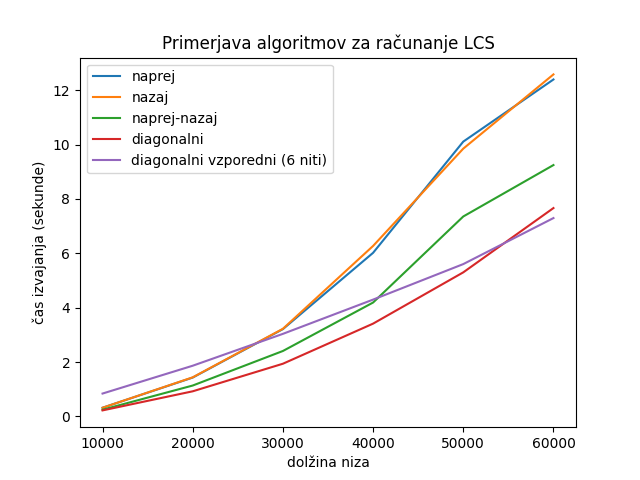
\includegraphics[width=1.0\textwidth]{plots/LCStotal.png}
\end{center}
\caption{Primerjava časov izvajanja LCS algoritmov brez prostorske optimizacije}
\label{comparison1}
\end{figure}

Pri primerjavi prostorsko optimiziranih funkcij (\ref{comparison2}) ravno tako vidimo, da ne obstaja bistvena razlika med pristopoma naprej in nazaj, je pa tukaj pristop naprej-nazaj res skoraj dvakrat hitrejši, iz česar lahko sklepamo, da je ozko grlo pri prenašanju dvodimenzionalnih tabel v predpomnilnik. 

Pri nizih dolžine približno 200000 začnemo opažati občutno razliko med tremi osnovnimi algoritmi (naprej, nazaj in diagonalno) in vzporednima algoritmoma (naprej-nazaj in diagonalno paralelno). Nekoliko presenetljiv rezultat je, da je tudi na relativno velikih dolžinah vhodnih podatkih pristop naprej-nazaj rahlo hitrejši od diagonalnega. Tukaj gre dejansko za primerjavo med algoritmom z dvema nitima, ki sta medseboj neodvisni (torej ločeno računata vsaka svojo polovico tabele) in algoritmom s šestimi nitmi, ki se morajo sinhronizirati na koncu vsake vrstice, pri čemer neizogibno pride do medsebojnega čakanja. 

\begin{figure}[htb]
\begin{center}
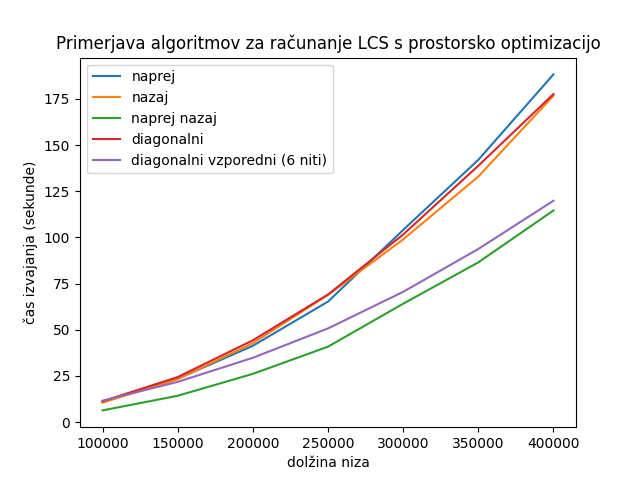
\includegraphics[width=1.0\textwidth]{plots/LCSspace.png}
\end{center}
\caption{Primerjava časov izvajanja LCS algoritmov s prostorsko optimizacijo}
\label{comparison2}
\end{figure}

\bigskip 
Vseeno pa smo pričakovali, da obstaja neka točka na kateri bo diagonalni algoritem postal hitrejši od naprej-nazaj, zato smo izvedli dodatne teste na še večjih dolžinah vhodnih nizov. Ker gre za metode s prostorsko optimizacijo tukaj nismo pretirano zaskrbljeni glede porabe pomnilnika: za tri enodimenzionalne tabele dolžine 700000 potrebujemo približno 8GB pomnilniškega prostora (če podatkovni tip int zasede 4 bajte v pomnilniku), kar je sprejemljivo za specifikacije naprave na kateri smo izvajali teste. 

Kot je razvidno iz slike (\ref{comparison3}), smo res našli točko kjer je cena sinhronizacije 6 niti dovolj majhna, da postane diagonalni algoritem hitejši od dveh neodvisnih niti - ta je približno med 500000 in 600000, pri 700000 pa je vzporedni algoritem hitrejši že za skoraj pol minute. 

\begin{figure}[htb]
\begin{center}
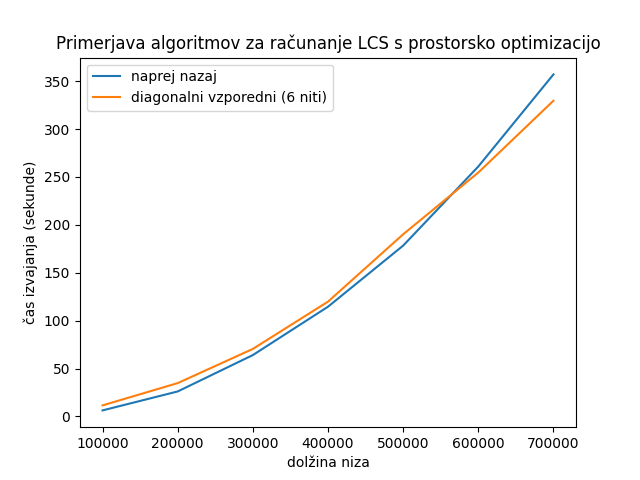
\includegraphics[width=1.0\textwidth]{plots/LCSextended.png}
\end{center}
\caption{Dodatna primerjava časov izvajanja LCS algoritmov s prostorsko optimizacijo}
\label{comparison3}
\end{figure}

\section{Primerjava algoritmov za Levenshteinovo razdaljo}

Ker sta algoritma za iskanje LCS in Levenshteinove razdalje konceptualno zelo podobna, lahko pričakujemo, da bo to razvidno tudi iz praktičnih meritev. Že na prvi pogled vidimo, da so razmerja med krivuljami res približno enaka (\ref{comparison4}). Dejanski časi izvajanja so tukaj nekoliko daljši, predvidoma zaradi gnezdenega klica funkcije $min()$, ki ni prisoten v algoritmu za računanje LCS. 

Zaradi daljših časov izvajanja se tudi izkaže, da občutimo uporabnost vzporednih algoritmov že na krajših dolžinah vhodnih nizov. Primer: pri LCS algoritmih (\ref{comparison1}) je osnovni diagonalni algoritem hitrejši od vzporednega do nizov dolžine približno 50000, pri Levenshteinovi razdalji (\ref{comparison4}) pa sta časa izvajanja približno enaka že pri nizih dolžine 40000. 

\begin{figure}[htb]
\begin{center}
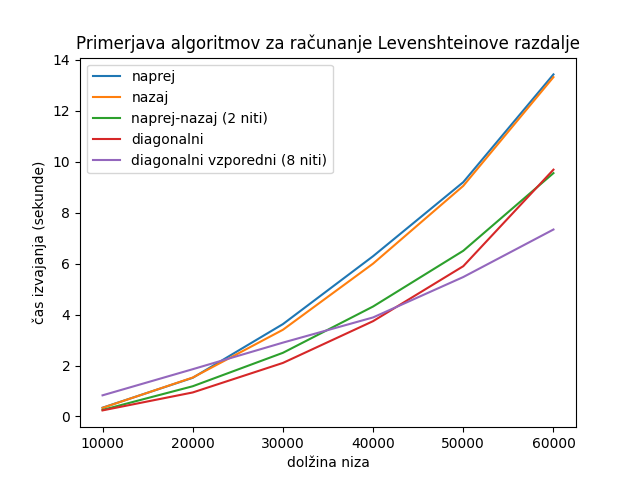
\includegraphics[width=1.0\textwidth]{plots/LevenshteinTotal.png}
\end{center}
\caption{Primerjava časov izvajanja algoritmov za iskanje Levenshteinove razdalje brez prostorske optimizacije}
\label{comparison4}
\end{figure}

Na tem mestu je smiselno, da si ogledamo še primerjavo časov izvajanja diagonalnega algoritma glede na število niti (\ref{comparison5}). Iz specifikacij sistema vemo, da lahko hkrati poganjamo največ 8 niti, vendar vidimo, da je tudi večje število niti (npr. 12) še vedno hitrejše od osnovnega algoritma. Ker pride v tem primeru do dodatnega čakanja med nitmi, seveda to ni smiselno, zato smo za meritve za Levenshteinovo razdaljo uporabljali 8 niti, za LCS pa se v povprečju bolje izkaže samo 6 niti. 

\begin{figure}[htb]
\begin{center}
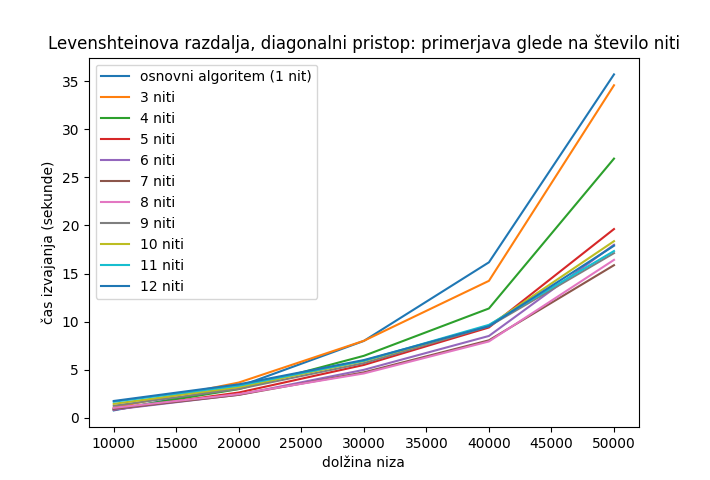
\includegraphics[width=1.0\textwidth]{plots/nThreads.png}
\end{center}
\caption{Primerjava časov izvajanja diagonalnih algoritmov glede na število niti}
\label{comparison5}
\end{figure}

Na sliki (\ref{comparison6}) je prikazana še primerjava časov izvajanja algoritmov s prostorsko optimizacijo. Ponovno vidimo, da je diagonalni vzporedni algoritem občutno hitrejši na bistveno krajših dolžinah nizov kot pri LCS (250000 proti 600000), zato tukaj niti ni potrebno, da izvajamo dodatne meritve nad dolžinami 400000. 

\begin{figure}[htb]
\begin{center}
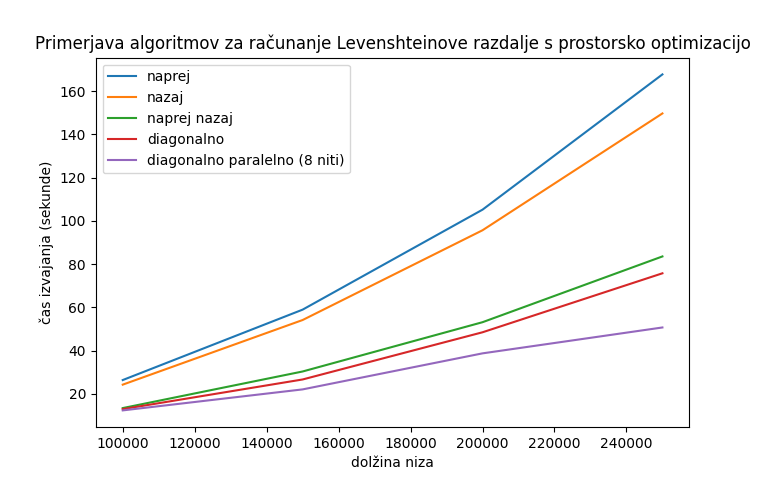
\includegraphics[width=1.0\textwidth]{plots/LevenshteinSpace.png}
\end{center}
\caption{Primerjava časov izvajanja algoritmov za iskanje Levenshteinove razdalje s prostorsko optimizacijo}
\label{comparison6}
\end{figure}

\chapter{Zaključki}

V tem poglavju predstavimo sklepne ugotovitve diplomskega dela in predlagamo nekaj možnih idej za nadaljnji razvoj.

\section{Sklepi}

Izkaže se, da obstajajo različni možni načini povzporejanja algoritmov za računanje dolžine LCS in Levenshteinove razdalje, kljub temu, da pri obeh problemih obstaja velika medsebojna odvisnost med izračunanimi rezultati v matriki. 

Veliko pohitritev dosežemo že z uporabo dveh niti, s pristopom naprej-nazaj. Izboljšave so vidne že na relativno majhnih vhodnih podatkih. Če nas zanima samo dolžina LCS ali Levenshteinove razdalje, in nas ne zanima rekonstrukcija poti, po kateri smo prišli do rezultata, pa lahko implementiramo še občutno izboljšano porabo prostora v pomnilniku, s tem da se izognemo uporabi dvodimenzionalnih matrik. Prostorsko zahtevnost tako izboljšamo iz $O(n^2)$ na $O(n)$. 

Za vzporedno izvajanje več kot dveh niti, se moramo poslužiti diagonalnega pristopa, pri katerem lahko izberemo poljubno število niti glede na omejitve strojne opreme na sistemu, na katerem se izvaja programska koda, ali pa glede na velikost vhodnih podatkov. 

\section{Nadaljnji razvoj}

Z vzporednimi algoritmi smo dosegli občutno pohitritev že na običajnih osebnih računalnikih. V nadaljnje bi bilo zanimivo preveriti ali je čas izvajanja morda še krajši na zmogljivejših sistemih z ogromno kolilčino jeder, oziroma ali je mogoče algoritme še dodatno prilagoditi za tovrstne sisteme. 

Zanimivo bi bilo tudi ugotoviti, ali je algoritme mogoče preurediti tako, da na nek način upoštevajo dolžine vhodnih nizov, predvsem če pride do situacije, ko je en niz bistveno krajši od drugega. Predvidevamo, da bi bilo v tem primeru smiselno krajši niz postaviti v vrstice, daljši niz pa v stolpce matrike, da bi s tem zmanjšali število sinhronizacij niti pri diagonalnem pristopu. 

%https://www.researchgate.net/publication/299366231_Computing_a_Longest_Common_Subsequence_for_Multiple_Sequences
%https://colab.ws/articles/10.1007%2F978-3-662-07675-0_8


%\cleardoublepage
%\addcontentsline{toc}{chapter}{Literatura}

% če imaš težave poravnati desni rob bibliografije, potem odkomentiraj spodnjo vrstico
\raggedright

%\printbibliography[heading=bibintoc,type=article,title={Članki v revijah}]

%\printbibliography[heading=bibintoc,type=inproceedings,title={Članki v zbornikih}]

%\printbibliography[heading=bibintoc,type=incollection,title={Poglavja v knjigah}]

% v zadnji verziji diplomskega dela običajno združiš vse tri vrste referenc v en sam seznam in
% izpustiš delne sezname
\printbibliography[heading=bibintoc,title={Literatura}]

\end{document}
